% Created by tikzDevice version 0.12 on 2020-05-15 20:00:00
% !TEX encoding = UTF-8 Unicode
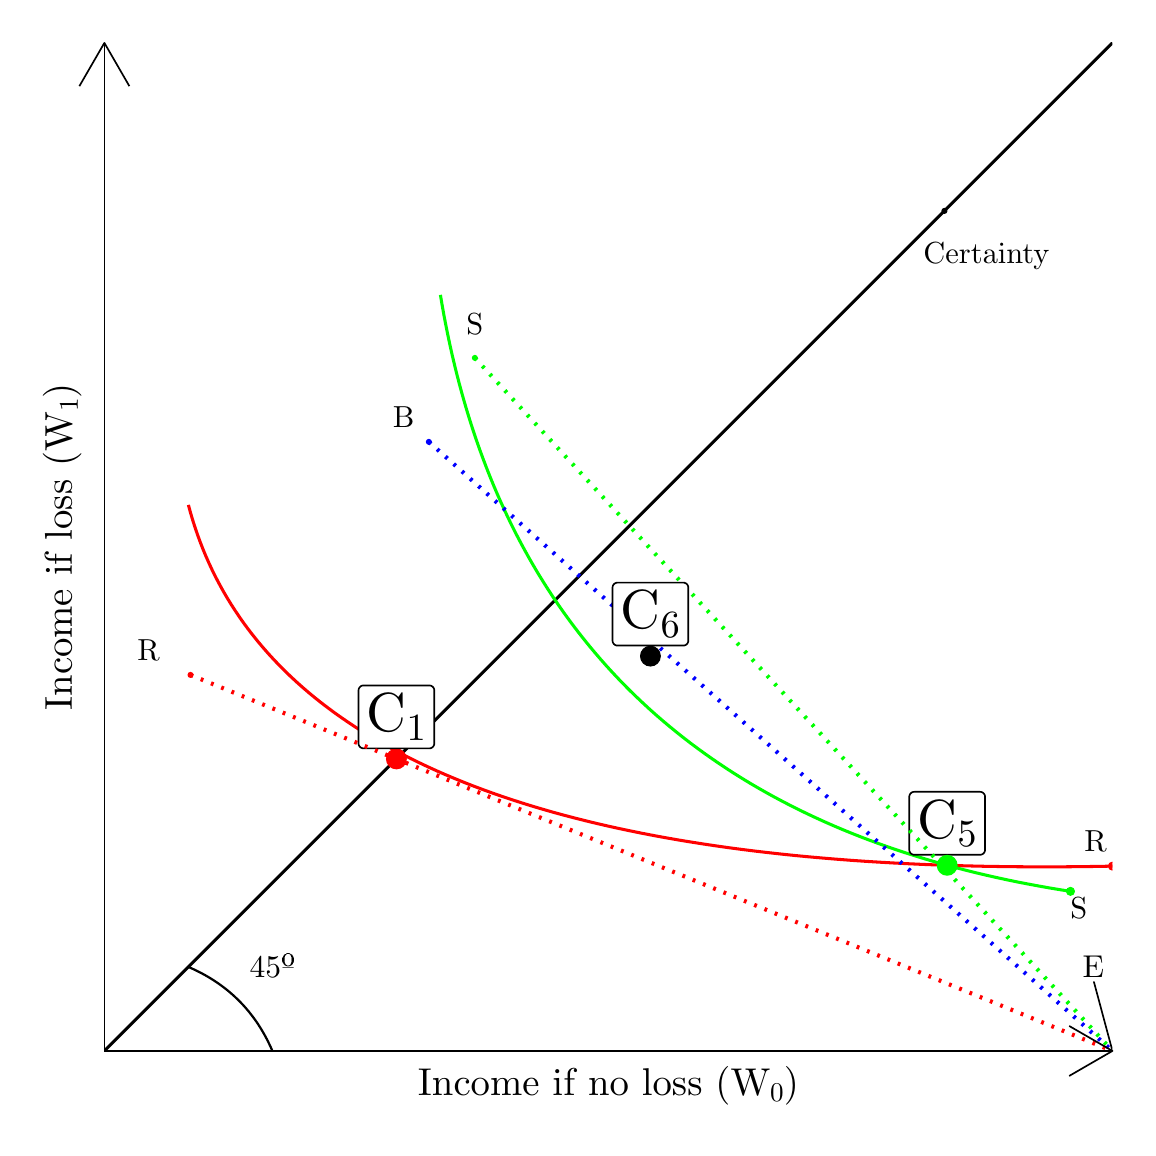
\begin{tikzpicture}[x=1pt,y=1pt]
\definecolor{fillColor}{RGB}{255,255,255}
\path[use as bounding box,fill=fillColor,fill opacity=0.00] (0,0) rectangle (397.48,397.48);
\begin{scope}
\path[clip] (  0.00,  0.00) rectangle (397.48,397.48);
\definecolor{drawColor}{RGB}{255,255,255}
\definecolor{fillColor}{RGB}{255,255,255}

\path[draw=drawColor,line width= 0.6pt,line join=round,line cap=round,fill=fillColor] (  0.00,  0.00) rectangle (397.48,397.48);
\end{scope}
\begin{scope}
\path[clip] ( 27.72, 27.72) rectangle (391.98,391.98);
\definecolor{fillColor}{RGB}{255,255,255}

\path[fill=fillColor] ( 27.72, 27.72) rectangle (391.98,391.98);
\definecolor{drawColor}{RGB}{0,0,0}

\path[draw=drawColor,line width= 1.1pt,line join=round] ( 27.72, 27.72) --
	( 31.40, 31.40) --
	( 35.08, 35.08) --
	( 38.76, 38.76) --
	( 42.44, 42.44) --
	( 46.12, 46.12) --
	( 49.79, 49.79) --
	( 53.47, 53.47) --
	( 57.15, 57.15) --
	( 60.83, 60.83) --
	( 64.51, 64.51) --
	( 68.19, 68.19) --
	( 71.87, 71.87) --
	( 75.55, 75.55) --
	( 79.23, 79.23) --
	( 82.91, 82.91) --
	( 86.59, 86.59) --
	( 90.27, 90.27) --
	( 93.95, 93.95) --
	( 97.63, 97.63) --
	(101.31,101.31) --
	(104.99,104.99) --
	(108.67,108.67) --
	(112.35,112.35) --
	(116.03,116.03) --
	(119.70,119.70) --
	(123.38,123.38) --
	(127.06,127.06) --
	(130.74,130.74) --
	(134.42,134.42) --
	(138.10,138.10) --
	(141.78,141.78) --
	(145.46,145.46) --
	(149.14,149.14) --
	(152.82,152.82) --
	(156.50,156.50) --
	(160.18,160.18) --
	(163.86,163.86) --
	(167.54,167.54) --
	(171.22,171.22) --
	(174.90,174.90) --
	(178.58,178.58) --
	(182.26,182.26) --
	(185.94,185.94) --
	(189.61,189.61) --
	(193.29,193.29) --
	(196.97,196.97) --
	(200.65,200.65) --
	(204.33,204.33) --
	(208.01,208.01) --
	(211.69,211.69) --
	(215.37,215.37) --
	(219.05,219.05) --
	(222.73,222.73) --
	(226.41,226.41) --
	(230.09,230.09) --
	(233.77,233.77) --
	(237.45,237.45) --
	(241.13,241.13) --
	(244.81,244.81) --
	(248.49,248.49) --
	(252.17,252.17) --
	(255.84,255.84) --
	(259.52,259.52) --
	(263.20,263.20) --
	(266.88,266.88) --
	(270.56,270.56) --
	(274.24,274.24) --
	(277.92,277.92) --
	(281.60,281.60) --
	(285.28,285.28) --
	(288.96,288.96) --
	(292.64,292.64) --
	(296.32,296.32) --
	(300.00,300.00) --
	(303.68,303.68) --
	(307.36,307.36) --
	(311.04,311.04) --
	(314.72,314.72) --
	(318.40,318.40) --
	(322.08,322.08) --
	(325.75,325.75) --
	(329.43,329.43) --
	(333.11,333.11) --
	(336.79,336.79) --
	(340.47,340.47) --
	(344.15,344.15) --
	(347.83,347.83) --
	(351.51,351.51) --
	(355.19,355.19) --
	(358.87,358.87) --
	(362.55,362.55) --
	(366.23,366.23) --
	(369.91,369.91) --
	(373.59,373.59) --
	(377.27,377.27) --
	(380.95,380.95) --
	(384.63,384.63) --
	(388.31,388.31) --
	(391.98,391.98);
\definecolor{drawColor}{RGB}{255,0,0}

\path[draw=drawColor,line width= 1.1pt,line join=round] ( 58.07,225.03) --
	( 58.82,222.28) --
	( 59.62,219.57) --
	( 60.48,216.88) --
	( 61.39,214.22) --
	( 62.35,211.60) --
	( 63.36,209.00) --
	( 64.43,206.43) --
	( 65.56,203.88) --
	( 66.73,201.37) --
	( 67.96,198.89) --
	( 69.25,196.44) --
	( 70.58,194.01) --
	( 71.98,191.61) --
	( 73.42,189.25) --
	( 74.92,186.91) --
	( 76.47,184.60) --
	( 78.07,182.32) --
	( 79.73,180.07) --
	( 81.45,177.85) --
	( 83.21,175.66) --
	( 85.03,173.50) --
	( 86.90,171.36) --
	( 88.83,169.26) --
	( 90.81,167.18) --
	( 92.84,165.14) --
	( 94.93,163.12) --
	( 97.07,161.13) --
	( 99.27,159.17) --
	(101.51,157.24) --
	(103.81,155.34) --
	(106.17,153.47) --
	(108.58,151.63) --
	(111.04,149.81) --
	(113.56,148.03) --
	(116.13,146.28) --
	(118.75,144.55) --
	(121.43,142.85) --
	(124.16,141.18) --
	(126.94,139.55) --
	(129.78,137.94) --
	(132.67,136.36) --
	(135.61,134.80) --
	(138.61,133.28) --
	(141.66,131.79) --
	(144.77,130.32) --
	(147.92,128.89) --
	(151.14,127.48) --
	(154.40,126.11) --
	(157.72,124.76) --
	(161.09,123.44) --
	(164.52,122.15) --
	(168.00,120.89) --
	(171.53,119.66) --
	(175.12,118.46) --
	(178.76,117.29) --
	(182.46,116.14) --
	(186.20,115.03) --
	(190.00,113.94) --
	(193.86,112.89) --
	(197.77,111.86) --
	(201.73,110.86) --
	(205.75,109.89) --
	(209.82,108.95) --
	(213.94,108.04) --
	(218.11,107.16) --
	(222.34,106.31) --
	(226.63,105.48) --
	(230.97,104.69) --
	(235.36,103.92) --
	(239.80,103.19) --
	(244.30,102.48) --
	(248.85,101.80) --
	(253.45,101.15) --
	(258.11,100.53) --
	(262.82, 99.94) --
	(267.59, 99.38) --
	(272.41, 98.85) --
	(277.28, 98.34) --
	(282.21, 97.87) --
	(287.19, 97.43) --
	(292.22, 97.01) --
	(297.31, 96.62) --
	(302.45, 96.26) --
	(307.64, 95.94) --
	(312.89, 95.64) --
	(318.19, 95.37) --
	(323.55, 95.12) --
	(328.96, 94.91) --
	(334.42, 94.73) --
	(339.93, 94.58) --
	(345.50, 94.45) --
	(351.13, 94.36) --
	(356.80, 94.29) --
	(362.53, 94.25) --
	(368.32, 94.24) --
	(374.15, 94.26) --
	(380.04, 94.31) --
	(385.99, 94.39) --
	(391.98, 94.50);
\definecolor{drawColor}{RGB}{0,255,0}

\path[draw=drawColor,line width= 1.1pt,line join=round] (149.14,300.92) --
	(149.77,297.19) --
	(150.43,293.50) --
	(151.13,289.84) --
	(151.87,286.21) --
	(152.63,282.61) --
	(153.43,279.04) --
	(154.27,275.51) --
	(155.14,272.00) --
	(156.04,268.53) --
	(156.98,265.09) --
	(157.95,261.68) --
	(158.95,258.30) --
	(159.99,254.96) --
	(161.06,251.64) --
	(162.17,248.36) --
	(163.31,245.11) --
	(164.49,241.89) --
	(165.70,238.70) --
	(166.94,235.55) --
	(168.22,232.42) --
	(169.53,229.33) --
	(170.88,226.27) --
	(172.26,223.24) --
	(173.67,220.24) --
	(175.12,217.27) --
	(176.60,214.34) --
	(178.12,211.43) --
	(179.67,208.56) --
	(181.25,205.72) --
	(182.87,202.91) --
	(184.52,200.13) --
	(186.21,197.39) --
	(187.93,194.67) --
	(189.68,191.99) --
	(191.47,189.34) --
	(193.29,186.72) --
	(195.15,184.13) --
	(197.04,181.58) --
	(198.97,179.05) --
	(200.93,176.56) --
	(202.92,174.10) --
	(204.95,171.67) --
	(207.01,169.27) --
	(209.10,166.90) --
	(211.23,164.57) --
	(213.39,162.27) --
	(215.59,159.99) --
	(217.82,157.75) --
	(220.09,155.55) --
	(222.39,153.37) --
	(224.72,151.22) --
	(227.09,149.11) --
	(229.49,147.03) --
	(231.93,144.98) --
	(234.40,142.96) --
	(236.90,140.97) --
	(239.44,139.01) --
	(242.01,137.09) --
	(244.62,135.20) --
	(247.26,133.34) --
	(249.93,131.51) --
	(252.64,129.71) --
	(255.38,127.94) --
	(258.16,126.21) --
	(260.97,124.50) --
	(263.82,122.83) --
	(266.70,121.19) --
	(269.61,119.58) --
	(272.56,118.01) --
	(275.54,116.46) --
	(278.55,114.95) --
	(281.60,113.47) --
	(284.68,112.02) --
	(287.80,110.60) --
	(290.95,109.21) --
	(294.14,107.85) --
	(297.36,106.53) --
	(300.61,105.24) --
	(303.90,103.98) --
	(307.22,102.75) --
	(310.58,101.55) --
	(313.97,100.38) --
	(317.39, 99.25) --
	(320.85, 98.15) --
	(324.34, 97.08) --
	(327.87, 96.04) --
	(331.43, 95.03) --
	(335.02, 94.05) --
	(338.65, 93.11) --
	(342.31, 92.19) --
	(346.01, 91.31) --
	(349.74, 90.46) --
	(353.50, 89.64) --
	(357.30, 88.85) --
	(361.14, 88.10) --
	(365.00, 87.38) --
	(368.90, 86.68) --
	(372.84, 86.02) --
	(376.81, 85.39);
\definecolor{drawColor}{RGB}{0,0,0}

\path[draw=drawColor,line width= 0.6pt,line join=round,line cap=round,fill=fillColor] (320.38, 98.61) --
	(344.14, 98.61) --
	(344.06, 98.61) --
	(344.35, 98.62) --
	(344.64, 98.68) --
	(344.91, 98.78) --
	(345.16, 98.93) --
	(345.39, 99.11) --
	(345.58, 99.33) --
	(345.74, 99.58) --
	(345.85, 99.84) --
	(345.92,100.13) --
	(345.94,100.42) --
	(345.94,100.42) --
	(345.94,119.54) --
	(345.94,119.54) --
	(345.92,119.83) --
	(345.85,120.12) --
	(345.74,120.38) --
	(345.58,120.63) --
	(345.39,120.85) --
	(345.16,121.03) --
	(344.91,121.18) --
	(344.64,121.28) --
	(344.35,121.34) --
	(344.14,121.35) --
	(320.38,121.35) --
	(320.59,121.34) --
	(320.30,121.35) --
	(320.01,121.31) --
	(319.73,121.23) --
	(319.47,121.11) --
	(319.23,120.94) --
	(319.02,120.74) --
	(318.85,120.51) --
	(318.71,120.25) --
	(318.62,119.98) --
	(318.57,119.69) --
	(318.57,119.54) --
	(318.57,100.42) --
	(318.57,100.56) --
	(318.57,100.27) --
	(318.62, 99.98) --
	(318.71, 99.71) --
	(318.85, 99.45) --
	(319.02, 99.22) --
	(319.23, 99.02) --
	(319.47, 98.85) --
	(319.73, 98.73) --
	(320.01, 98.64) --
	(320.30, 98.61) --
	cycle;
\end{scope}
\begin{scope}
\path[clip] ( 27.72, 27.72) rectangle (391.98,391.98);
\definecolor{drawColor}{RGB}{0,0,0}

\node[text=drawColor,anchor=base west,inner sep=0pt, outer sep=0pt, scale=  1.99] at (321.58,104.62) {C};

\node[text=drawColor,anchor=base west,inner sep=0pt, outer sep=0pt, scale=  1.39] at (335.96,101.62) {5};
\definecolor{drawColor}{RGB}{0,255,0}
\definecolor{fillColor}{RGB}{0,255,0}

\path[draw=drawColor,line width= 0.4pt,line join=round,line cap=round,fill=fillColor] (332.26, 94.80) circle (  3.57);
\definecolor{drawColor}{RGB}{255,0,0}
\definecolor{fillColor}{RGB}{255,0,0}

\path[draw=drawColor,line width= 0.4pt,line join=round,line cap=round,fill=fillColor] (133.24,133.24) circle (  3.57);
\definecolor{drawColor}{RGB}{0,0,0}
\definecolor{fillColor}{RGB}{255,255,255}

\path[draw=drawColor,line width= 0.6pt,line join=round,line cap=round,fill=fillColor] (121.36,137.05) --
	(145.12,137.05) --
	(145.05,137.05) --
	(145.34,137.06) --
	(145.63,137.12) --
	(145.90,137.22) --
	(146.15,137.37) --
	(146.37,137.55) --
	(146.57,137.77) --
	(146.72,138.02) --
	(146.84,138.28) --
	(146.91,138.57) --
	(146.93,138.86) --
	(146.93,138.86) --
	(146.93,157.99) --
	(146.93,157.99) --
	(146.91,158.27) --
	(146.84,158.56) --
	(146.72,158.82) --
	(146.57,159.07) --
	(146.37,159.29) --
	(146.15,159.47) --
	(145.90,159.62) --
	(145.63,159.72) --
	(145.34,159.78) --
	(145.12,159.79) --
	(121.36,159.79) --
	(121.58,159.78) --
	(121.29,159.79) --
	(121.00,159.76) --
	(120.72,159.67) --
	(120.46,159.55) --
	(120.22,159.38) --
	(120.01,159.18) --
	(119.84,158.95) --
	(119.70,158.69) --
	(119.61,158.42) --
	(119.56,158.13) --
	(119.56,157.99) --
	(119.56,138.86) --
	(119.56,139.00) --
	(119.56,138.71) --
	(119.61,138.42) --
	(119.70,138.15) --
	(119.84,137.89) --
	(120.01,137.66) --
	(120.22,137.46) --
	(120.46,137.29) --
	(120.72,137.17) --
	(121.00,137.09) --
	(121.29,137.05) --
	cycle;
\end{scope}
\begin{scope}
\path[clip] ( 27.72, 27.72) rectangle (391.98,391.98);
\definecolor{drawColor}{RGB}{0,0,0}

\node[text=drawColor,anchor=base west,inner sep=0pt, outer sep=0pt, scale=  1.99] at (122.57,143.06) {C};

\node[text=drawColor,anchor=base west,inner sep=0pt, outer sep=0pt, scale=  1.39] at (136.95,140.06) {1};
\definecolor{drawColor}{RGB}{255,0,0}

\path[draw=drawColor,line width= 1.5pt,dash pattern=on 1pt off 3pt ,line join=round] ( 58.83,163.59) --
	(391.98, 27.72);
\definecolor{drawColor}{RGB}{0,255,0}

\path[draw=drawColor,line width= 1.5pt,dash pattern=on 1pt off 3pt ,line join=round] (161.59,278.15) --
	(391.98, 27.72);
\definecolor{drawColor}{RGB}{0,0,255}

\path[draw=drawColor,line width= 1.5pt,dash pattern=on 1pt off 3pt ,line join=round] (144.97,247.80) --
	(391.98, 27.72);
\definecolor{drawColor}{RGB}{0,0,0}

\path[draw=drawColor,line width= 0.8pt,line join=round] ( 58.07, 58.07) --
	( 58.50, 57.89) --
	( 58.93, 57.70) --
	( 59.35, 57.51) --
	( 59.77, 57.32) --
	( 60.19, 57.12) --
	( 60.60, 56.93) --
	( 61.02, 56.73) --
	( 61.43, 56.52) --
	( 61.84, 56.32) --
	( 62.24, 56.11) --
	( 62.65, 55.90) --
	( 63.05, 55.69) --
	( 63.44, 55.47) --
	( 63.84, 55.26) --
	( 64.23, 55.04) --
	( 64.62, 54.81) --
	( 65.01, 54.59) --
	( 65.40, 54.36) --
	( 65.78, 54.13) --
	( 66.16, 53.90) --
	( 66.54, 53.66) --
	( 66.92, 53.43) --
	( 67.29, 53.19) --
	( 67.66, 52.94) --
	( 68.03, 52.70) --
	( 68.40, 52.45) --
	( 68.76, 52.20) --
	( 69.12, 51.95) --
	( 69.48, 51.70) --
	( 69.84, 51.44) --
	( 70.19, 51.18) --
	( 70.54, 50.92) --
	( 70.89, 50.65) --
	( 71.24, 50.39) --
	( 71.58, 50.12) --
	( 71.92, 49.85) --
	( 72.26, 49.57) --
	( 72.60, 49.29) --
	( 72.93, 49.01) --
	( 73.26, 48.73) --
	( 73.59, 48.45) --
	( 73.92, 48.16) --
	( 74.24, 47.87) --
	( 74.56, 47.58) --
	( 74.88, 47.29) --
	( 75.20, 46.99) --
	( 75.51, 46.69) --
	( 75.82, 46.39) --
	( 76.13, 46.08) --
	( 76.44, 45.78) --
	( 76.74, 45.47) --
	( 77.05, 45.16) --
	( 77.34, 44.84) --
	( 77.64, 44.53) --
	( 77.94, 44.21) --
	( 78.23, 43.89) --
	( 78.52, 43.56) --
	( 78.80, 43.24) --
	( 79.09, 42.91) --
	( 79.37, 42.58) --
	( 79.65, 42.24) --
	( 79.93, 41.91) --
	( 80.20, 41.57) --
	( 80.47, 41.22) --
	( 80.74, 40.88) --
	( 81.01, 40.53) --
	( 81.27, 40.19) --
	( 81.54, 39.83) --
	( 81.80, 39.48) --
	( 82.05, 39.13) --
	( 82.31, 38.77) --
	( 82.56, 38.41) --
	( 82.81, 38.04) --
	( 83.06, 37.68) --
	( 83.30, 37.31) --
	( 83.54, 36.94) --
	( 83.78, 36.56) --
	( 84.02, 36.19) --
	( 84.25, 35.81) --
	( 84.49, 35.43) --
	( 84.72, 35.04) --
	( 84.94, 34.66) --
	( 85.17, 34.27) --
	( 85.39, 33.88) --
	( 85.61, 33.49) --
	( 85.83, 33.09) --
	( 86.04, 32.69) --
	( 86.26, 32.29) --
	( 86.47, 31.89) --
	( 86.67, 31.48) --
	( 86.88, 31.07) --
	( 87.08, 30.66) --
	( 87.28, 30.25) --
	( 87.48, 29.83) --
	( 87.67, 29.42) --
	( 87.87, 28.99) --
	( 88.06, 28.57) --
	( 88.24, 28.15) --
	( 88.43, 27.72);

\node[text=drawColor,anchor=base,inner sep=0pt, outer sep=0pt, scale=  1.14] at ( 88.43, 54.15) {45º};

\path[draw=drawColor,line width= 0.6pt,line join=round,line cap=round] (385.29, 52.65) -- (391.98, 27.72);

\node[text=drawColor,anchor=base,inner sep=0pt, outer sep=0pt, scale=  1.14] at (385.10, 54.15) {E};
\definecolor{fillColor}{RGB}{0,0,0}

\path[draw=drawColor,line width= 0.4pt,line join=round,line cap=round,fill=fillColor] (225.03,170.39) circle (  3.57);
\definecolor{fillColor}{RGB}{255,255,255}

\path[draw=drawColor,line width= 0.6pt,line join=round,line cap=round,fill=fillColor] (213.15,174.20) --
	(236.91,174.20) --
	(236.84,174.20) --
	(237.13,174.21) --
	(237.41,174.27) --
	(237.68,174.37) --
	(237.94,174.52) --
	(238.16,174.70) --
	(238.35,174.92) --
	(238.51,175.16) --
	(238.62,175.43) --
	(238.69,175.71) --
	(238.72,176.00) --
	(238.72,176.00) --
	(238.72,195.13) --
	(238.72,195.13) --
	(238.69,195.42) --
	(238.62,195.70) --
	(238.51,195.97) --
	(238.35,196.22) --
	(238.16,196.43) --
	(237.94,196.62) --
	(237.68,196.76) --
	(237.41,196.87) --
	(237.13,196.93) --
	(236.91,196.94) --
	(213.15,196.94) --
	(213.37,196.93) --
	(213.08,196.94) --
	(212.79,196.90) --
	(212.51,196.82) --
	(212.25,196.70) --
	(212.01,196.53) --
	(211.80,196.33) --
	(211.62,196.10) --
	(211.49,195.84) --
	(211.39,195.56) --
	(211.35,195.28) --
	(211.34,195.13) --
	(211.34,176.00) --
	(211.35,176.15) --
	(211.35,175.86) --
	(211.39,175.57) --
	(211.49,175.29) --
	(211.62,175.04) --
	(211.80,174.80) --
	(212.01,174.60) --
	(212.25,174.44) --
	(212.51,174.31) --
	(212.79,174.23) --
	(213.08,174.20) --
	cycle;
\end{scope}
\begin{scope}
\path[clip] ( 27.72, 27.72) rectangle (391.98,391.98);
\definecolor{drawColor}{RGB}{0,0,0}

\node[text=drawColor,anchor=base west,inner sep=0pt, outer sep=0pt, scale=  1.99] at (214.35,180.21) {C};

\node[text=drawColor,anchor=base west,inner sep=0pt, outer sep=0pt, scale=  1.39] at (228.74,177.21) {6};
\definecolor{drawColor}{RGB}{255,0,0}
\definecolor{fillColor}{RGB}{255,0,0}

\path[draw=drawColor,line width= 0.4pt,line join=round,line cap=round,fill=fillColor] (391.98, 94.50) circle (  1.43);
\definecolor{drawColor}{RGB}{0,0,0}

\node[text=drawColor,anchor=base,inner sep=0pt, outer sep=0pt, scale=  1.10] at (385.91, 99.81) {R};
\definecolor{drawColor}{RGB}{0,255,0}
\definecolor{fillColor}{RGB}{0,255,0}

\path[draw=drawColor,line width= 0.4pt,line join=round,line cap=round,fill=fillColor] (376.81, 85.39) circle (  1.43);
\definecolor{drawColor}{RGB}{0,0,0}

\node[text=drawColor,anchor=base,inner sep=0pt, outer sep=0pt, scale=  1.10] at (379.84, 75.52) {S};
\definecolor{fillColor}{RGB}{0,0,0}

\path[draw=drawColor,line width= 0.4pt,line join=round,line cap=round,fill=fillColor] (331.27,331.27) circle (  0.89);

\node[text=drawColor,anchor=base,inner sep=0pt, outer sep=0pt, scale=  1.10] at (346.45,312.29) {Certainty};
\definecolor{drawColor}{RGB}{255,0,0}
\definecolor{fillColor}{RGB}{255,0,0}

\path[draw=drawColor,line width= 0.4pt,line join=round,line cap=round,fill=fillColor] ( 58.83,163.59) circle (  0.89);
\definecolor{drawColor}{RGB}{0,0,0}

\node[text=drawColor,anchor=base,inner sep=0pt, outer sep=0pt, scale=  1.10] at ( 43.65,168.89) {R};
\definecolor{drawColor}{RGB}{0,255,0}
\definecolor{fillColor}{RGB}{0,255,0}

\path[draw=drawColor,line width= 0.4pt,line join=round,line cap=round,fill=fillColor] (161.59,278.15) circle (  0.89);
\definecolor{drawColor}{RGB}{0,0,0}

\node[text=drawColor,anchor=base,inner sep=0pt, outer sep=0pt, scale=  1.10] at (161.59,286.49) {S};
\definecolor{drawColor}{RGB}{0,0,255}
\definecolor{fillColor}{RGB}{0,0,255}

\path[draw=drawColor,line width= 0.4pt,line join=round,line cap=round,fill=fillColor] (144.97,247.80) circle (  0.89);
\definecolor{drawColor}{RGB}{0,0,0}

\node[text=drawColor,anchor=base,inner sep=0pt, outer sep=0pt, scale=  1.10] at (135.86,253.10) {B};
\end{scope}
\begin{scope}
\path[clip] (  0.00,  0.00) rectangle (397.48,397.48);
\definecolor{drawColor}{RGB}{0,0,0}

\path[draw=drawColor,line width= 0.6pt,line join=round] ( 27.72, 27.72) --
	( 27.72,391.98);

\path[draw=drawColor,line width= 0.6pt,line join=round] ( 36.75,376.34) --
	( 27.72,391.98) --
	( 18.68,376.34);
\end{scope}
\begin{scope}
\path[clip] (  0.00,  0.00) rectangle (397.48,397.48);
\definecolor{drawColor}{RGB}{0,0,0}

\path[draw=drawColor,line width= 0.6pt,line join=round] ( 27.72, 27.72) --
	(391.98, 27.72);

\path[draw=drawColor,line width= 0.6pt,line join=round] (376.34, 18.68) --
	(391.98, 27.72) --
	(376.34, 36.75);
\end{scope}
\begin{scope}
\path[clip] (  0.00,  0.00) rectangle (397.48,397.48);
\definecolor{drawColor}{RGB}{0,0,0}

\node[text=drawColor,anchor=base west,inner sep=0pt, outer sep=0pt, scale=  1.40] at (141.04, 11.72) {Income if no loss (W};

\node[text=drawColor,anchor=base west,inner sep=0pt, outer sep=0pt, scale=  0.98] at (268.33,  9.61) {0};

\node[text=drawColor,anchor=base west,inner sep=0pt, outer sep=0pt, scale=  1.40] at (273.22, 11.72) {)};
\end{scope}
\begin{scope}
\path[clip] (  0.00,  0.00) rectangle (397.48,397.48);
\definecolor{drawColor}{RGB}{0,0,0}

\node[text=drawColor,rotate= 90.00,anchor=base west,inner sep=0pt, outer sep=0pt, scale=  1.40] at ( 16.00,150.76) {Income if loss (W};

\node[text=drawColor,rotate= 90.00,anchor=base west,inner sep=0pt, outer sep=0pt, scale=  0.98] at ( 18.11,258.61) {1};

\node[text=drawColor,rotate= 90.00,anchor=base west,inner sep=0pt, outer sep=0pt, scale=  1.40] at ( 16.00,263.50) {)};
\end{scope}
\end{tikzpicture}
